\section{Background}
Understanding the relationship between cell resolution ($dx$) and model run time is extremely helpful when designing future numerical experiments.
This relationship has been hypothesized, but is unknown with regards to the \textit{pyDeltaRCM} model (at the time of writing). 

\section{Model Runs}
A set of 6 model runs, each with a different cell resolution ($dx$) are conducted.
These runs are at ``field-scale" using parameters similar to those from previous studies \cite{Liang2016, Liang2016a}.
The YAML below provides information about the parameter set used.\\

\noindent \texttt{YAML} configuration file: \vspace{-6pt}
\begin{boxedverbatim}
timesteps: 5000
Length: 7500.0
Width: 15000.0
L0_meters: 150.0
N0_meters: 250.0
h0: 5.0
SLR: 36e-10  # small background SLR
Np_water: 2000
Np_sed: 2000
save_dt: 250000

matrix:
  dx:
    - 25.0
    - 30.0
    - 40.0
    - 50.0
    - 75.0
    - 100.0
\end{boxedverbatim}

\section{Results}
Run time is plotted as a function of cell size and as a function of the total number of grids in the domain (Figure \ref{fig:res_v_runtime}). 

\begin{figure}[!ht]
	\makebox[\textwidth][c]{
	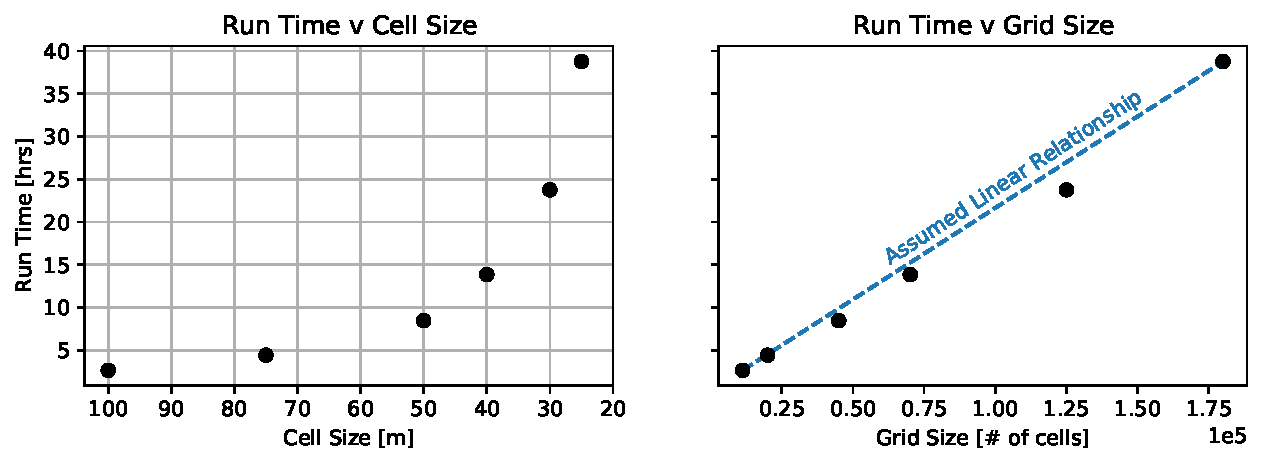
\includegraphics[width=\textwidth]{CellResRuntime/figs/RunTime_v_CellSize_naive.pdf}
	}	
	\caption{Results from the 6 runs generated by the YAML configuration file. \textit{Left:} Run time as a function of cell size. \textit{Right:} Run time as a function of the total number of cells in the domain.}
	\label{fig:res_v_runtime}
\end{figure}

\section{Conclusions}
There appears to be a linear relationship between the total number of grid cells in the domain and the runtime, and a nonlinear relationship between the cell resolution ($dx$) and runtime.
This finding is consistent, as the number of cells in a domain of fixed size scales inversely with the resolution of the individual cells ($dx$):

\begin{equation}
\text{\# cells} \sim \frac{1}{dx^2}
\end{equation}

Meaning that when the cell size is increased, the number of individual cells within the domain is reduced, and model runtime decreases. Conversely, when the cell resolution is increased, the number of cells increases, as does model runtime.

\clearpage
\bibliographystyle{plainnat}
\bibliography{bib/bib}